% Don't touch this %%%%%%%%%%%%%%%%%%%%%%%%%%%%%%%%%%%%%%%%%%%
\documentclass[11pt]{article}
\usepackage{fullpage}
\usepackage[left=1in,top=1in,right=1in,bottom=1in,headheight=3ex,headsep=3ex]{geometry}
\usepackage{graphicx}
\usepackage{float}
\renewcommand{\theenumi}{\Alph{enumi})}

\newcommand{\blankline}{\quad\pagebreak[2]}
%%%%%%%%%%%%%%%%%%%%%%%%%%%%%%%%%%%%%%%%%%%%%%%%%%%%%%%%%%%%%%

% Modify Course title, instructor name, semester here %%%%%%%%

\title{\textbf{GGR424: Transportation Geography \& Planning}}
\author{Jeff Allen}
\date{Winter, 2022}

%%%%%%%%%%%%%%%%%%%%%%%%%%%%%%%%%%%%%%%%%%%%%%%%%%%%%%%%%%%%%%

% Don't touch this %%%%%%%%%%%%%%%%%%%%%%%%%%%%%%%%%%%%%%%%%%%
\usepackage[sc]{mathpazo}
\linespread{1.05} % Palatino needs more leading (space between lines)
\usepackage[T1]{fontenc}
\usepackage[mmddyyyy]{datetime}% http://ctan.org/pkg/datetime
\usepackage{advdate}% http://ctan.org/pkg/advdate
\newdateformat{syldate}{\twodigit{\THEMONTH}/\twodigit{\THEDAY}}
\newsavebox{\MONDAY}\savebox{\MONDAY}{Mon}% Mon
\newcommand{\week}[1]{%
	%  \cleardate{mydate}% Clear date
	% \newdate{mydate}{\the\day}{\the\month}{\the\year}% Store date
	\paragraph*{\kern-2ex\quad #1, \syldate{\today} - \AdvanceDate[4]\syldate{\today}:}% Set heading  \quad #1
	%  \setbox1=\hbox{\shortdayofweekname{\getdateday{mydate}}{\getdatemonth{mydate}}{\getdateyear{mydate}}}%
	\ifdim\wd1=\wd\MONDAY
	\AdvanceDate[7]
	\else
	\AdvanceDate[7]
	\fi%
}
\usepackage{setspace}
\usepackage{multicol}
%\usepackage{indentfirst}
\usepackage{fancyhdr,lastpage}
\usepackage{url}
\pagestyle{fancy}
\usepackage{hyperref}
\usepackage{lastpage}
\usepackage{amsmath}
\usepackage{layout}

\lhead{}
\chead{}
%%%%%%%%%%%%%%%%%%%%%%%%%%%%%%%%%%%%%%%%%%%%%%%%%%%%%%%%%%%%%%

% Modify header here %%%%%%%%%%%%%%%%%%%%%%%%%%%%%%%%%%%%%%%%%
\rhead{\footnotesize Quiz 1 | GGR424}
\lhead{\footnotesize Jeff Allen}
%%%%%%%%%%%%%%%%%%%%%%%%%%%%%%%%%%%%%%%%%%%%%%%%%%%%%%%%%%%%%%
% Don't touch this %%%%%%%%%%%%%%%%%%%%%%%%%%%%%%%%%%%%%%%%%%%
\lfoot{}
\cfoot{\small \thepage/\pageref*{LastPage}}
\rfoot{}

\usepackage{array, xcolor}
\usepackage{color,hyperref}
\definecolor{clemsonorange}{HTML}{f00000}
\hypersetup{colorlinks,breaklinks,linkcolor=clemsonorange,urlcolor=clemsonorange,anchorcolor=clemsonorange,citecolor=black}

\setlength{\parindent}{0em}
\setlength{\parskip}{0.8em}

\usepackage{colortbl}
\usepackage{tabularx,ragged2e}
\usepackage{sectsty}


\usepackage{helvet}

\begin{document}
	\allsectionsfont{\sffamily}
		
	\textit{Due February 11 at 11:59pm}
		
	\section*{Quiz 1}
	
	Consider a city with 10 neighbourhoods that are connected with a single transit line. Assume that the travel time between each adjacent stop is \textbf{10 minutes} and that the headway is \textbf{2 minutes}.
	
	\begin{figure}[h]
		\centering
		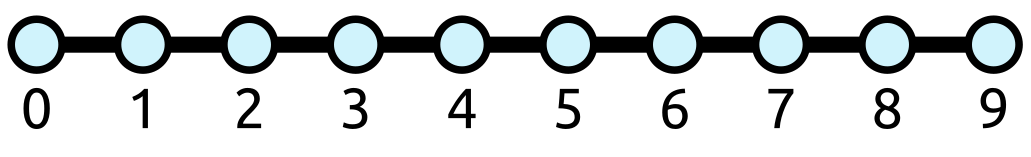
\includegraphics[width=0.5\linewidth]{images/city_plain.png}
	\end{figure}

	Use your student number to distribute where employment is located in the city. Do this by allocating 1,000 jobs to each neighbourhood for each digit in your student number.
	
	For example, if your student number is 1023455888, then the distribution of jobs in the city would be as follows:
	
	\begin{figure}[h]
		\centering
		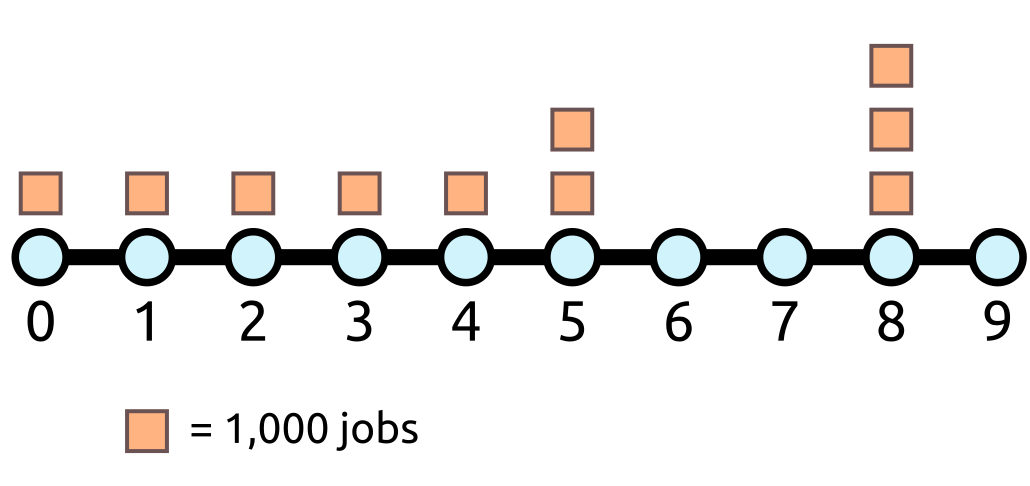
\includegraphics[width=0.5\linewidth]{images/city_jobs.png}
	\end{figure}
	
	Answer the following on Quercus based on your student number:
	
	\begin{enumerate}
		
		\item State your student number
		
		\item If you live in neighbourhood \textbf{0}, how many jobs can you reach in less than or equal to a \textbf{45} minute transit trip?
		
		\item Using this travel time threshold (\textbf{45} minutes), which neighbourhood(s) has the greatest level of accessibility to jobs?
		
		\item Pretend that the city is building a high speed express route to directly connect neighbourhood \textbf{0} and neighbourhood \textbf{9} in only \textbf{30} minutes and with a headway of \textbf{2} minutes. If you still live in neighbourhood \textbf{0}, how many jobs will you then be able to access in a \textbf{45} minute trip?
		
	\end{enumerate}
	
	
	
	
\end{document}